\chapter{Results}
\label{ch:results}

This chapter reports what happened when the four agents were run on historical data. Numbers first, mechanism second. Section~\ref{sec:experimental_setup} names the four agents in plain English. Section~\ref{sec:forecast_uncertainty} shows the confidence signal and checks that the forecaster is calibrated. Section~\ref{sec:headline_aggregate} is the SPY case study. Sections~\ref{sec:phase2_full_grid}--\ref{sec:phase2_inference} scale to 70 stocks with statistical tests. Section~\ref{sec:ablation} asks which half of the design (state, guard, or scaling) does the work. Section~\ref{sec:walk_forward} tests earlier time periods. Section~\ref{sec:phase2_interpretation} states honest limits.

\section{Experimental setup}
\label{sec:experimental_setup}

All numbers below are evaluated on held-out test windows. For the main grid (Sections~\ref{sec:headline_aggregate}--\ref{sec:phase2_full_grid}), the test window is 1 January 2022 to 31 December 2025. For walk-forward validation (Section~\ref{sec:walk_forward}), four non-overlapping two-year test windows cover 2018--2025.

The experiment compares four strategies on the same stocks, dates, and random seeds:

\begin{itemize}[leftmargin=*]
  \item \textbf{Arm~A --- Plain PPO (control).} A standard learning agent with \emph{no} forecaster and \emph{no} confidence signal. Shows what happens when the agent must trade blind to forecast confidence.
  \item \textbf{Arm~B --- PPO + market-noise signal (aleatoric).} The forecaster outputs a mean and a spread each day; the spread becomes the confidence signal. High signal means the market itself looks chaotic; the agent trades smaller or stops buying.
  \item \textbf{Arm~C --- PPO + model-unfamiliarity signal (epistemic).} The same setup, but confidence comes from running the forecaster twenty times with random dropout (Monte-Carlo dropout). High signal means today's data look unlike the training years; the same shrink-and-guard rules apply.
\end{itemize}

Each run trains one agent on one stock with one random seed. At full scale: 70 stocks $\times$ 10 seeds $\times$ 50{,}000 learning steps per cell, starting from \$1{,}000{,}000.

\section{Forecast uncertainty in the test window}
\label{sec:forecast_uncertainty}

Figure~\ref{fig:uncertainty_signal} shows the normalised uncertainty score $u_t$ that the probabilistic agent reads as part of its state, in the aleatoric mode of Section~\ref{sec:aleatoric_mode}. The high-uncertainty bands cluster around regions of elevated realised volatility, which is what one would hope to see if the forecaster has learned anything useful. Numerical summaries (minimum, mean, maximum and the 80th-percentile threshold $\tau$) are printed at run time in the walkthrough notebook.

\begin{figure}[h]
\centering
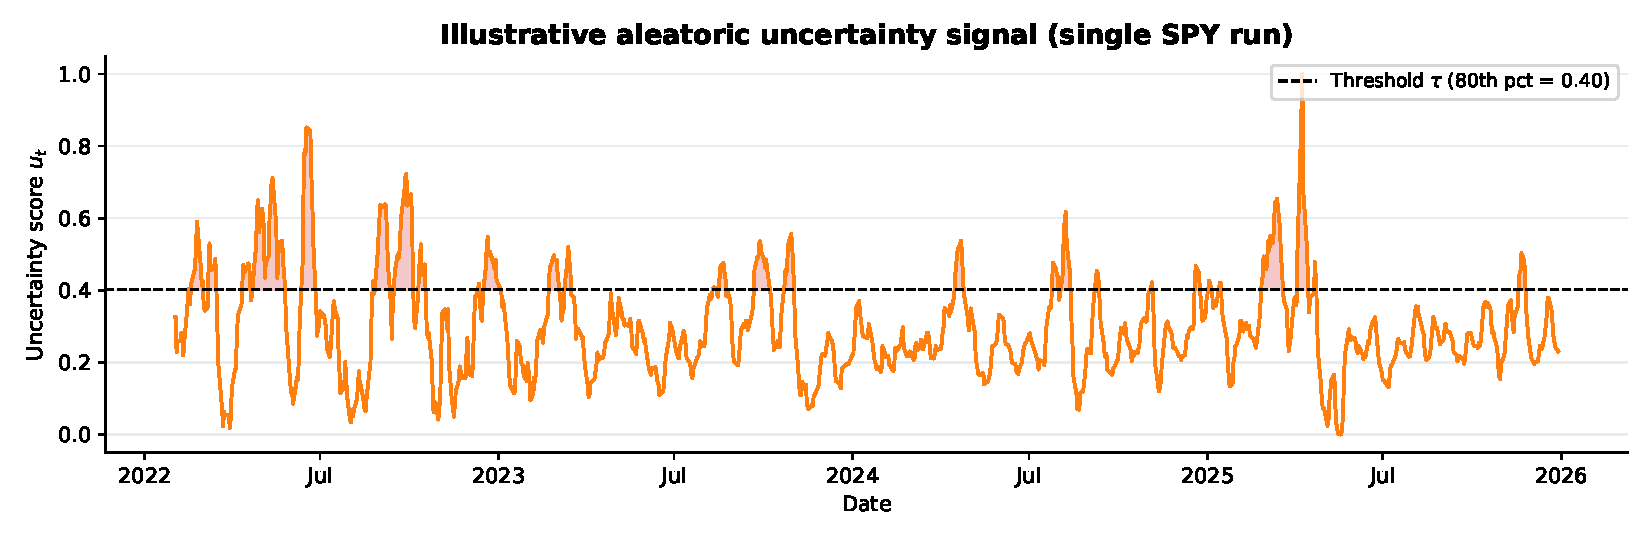
\includegraphics[width=0.95\textwidth]{../reports/generated/charts/uncertainty_signal.pdf}
\caption{Normalised aleatoric uncertainty score $u_t$ on the SPY test window. The horizontal dashed line is the 80th-percentile threshold $\tau$; new long-side trades are blocked on days where $u_t \geq \tau$.}
\label{fig:uncertainty_signal}
\end{figure}

The epistemic-mode uncertainty score from Equation~\ref{eq:epistemic_uncertainty} is computed alongside the aleatoric score in the walkthrough notebook. The empirical correlation between the two signals on the SPY test window is about $0.05$ --- close to zero, which is informative and confirms that the two scores capture distinct quantities. The two signals measure genuinely different things: aleatoric measures data-noise (``how chaotic is the market right now?''), while epistemic measures model unfamiliarity (``how different from the training distribution does today look?''). Section~\ref{sec:phase2_full_grid} reports the empirical consequence for the trained agent across the full market sample.

\subsection{Is the uncertainty signal calibrated?}
\label{sec:forecaster_calibration}

The trade-scaling factor and the risk-on guard of Equation~\ref{eq:probabilistic_trade_size} both treat the forecaster's predictive variance as a meaningful quantity. If the forecaster were systematically over-confident or under-confident the policy would be reading a free parameter, not an uncertainty signal. The check is the standard one: train the forecaster on the training window (2009--2018), predict on the held-out validation window (2019--2021), and ask how often the realised return falls inside the predicted central interval at each nominal level. The script is committed at \texttt{reports/builders/build\_forecaster\_calibration.py} and re-runs in under a minute on a single CPU core.

Figure~\ref{fig:forecaster_calibration} reports the result. The reliability diagram on the left puts the nominal coverage on the horizontal axis and the empirical coverage on the vertical axis; a perfectly calibrated forecaster lies on the dashed diagonal. The SPY forecaster sits on the diagonal up to the 80th-percentile mark and drifts very slightly below it on the tail (coverage at nominal 95\,\% is 92.2\,\%, the known signature of a Gaussian-head forecaster on heavy-tailed returns; \textcite{cont2001empirical}). Critically, the empirical coverage at the nominal 80\,\% level is 81.0\,\% --- which is the level at which the threshold $\tau$ is set --- so the guard fires on the days the forecaster genuinely flags as the top quintile of uncertainty. The Expected Calibration Error~\parencite{guo2017calibration} across the full curve is 0.045, well below the 0.10 figure typical of modern over-confident deep networks. The right panel of Figure~\ref{fig:forecaster_calibration} shows the per-day absolute residual against the predicted standard deviation: residuals scale linearly with $\hat\sigma_t$, confirming that the variance head tracks the realised noise level rather than emitting a constant. The validation NLL is $-3.63$ and the RMSE on next-day log returns is $0.0141$ (1.4\,\%), in line with what a small probabilistic LSTM should achieve on a broad-market index.

\begin{figure}[h]
\centering
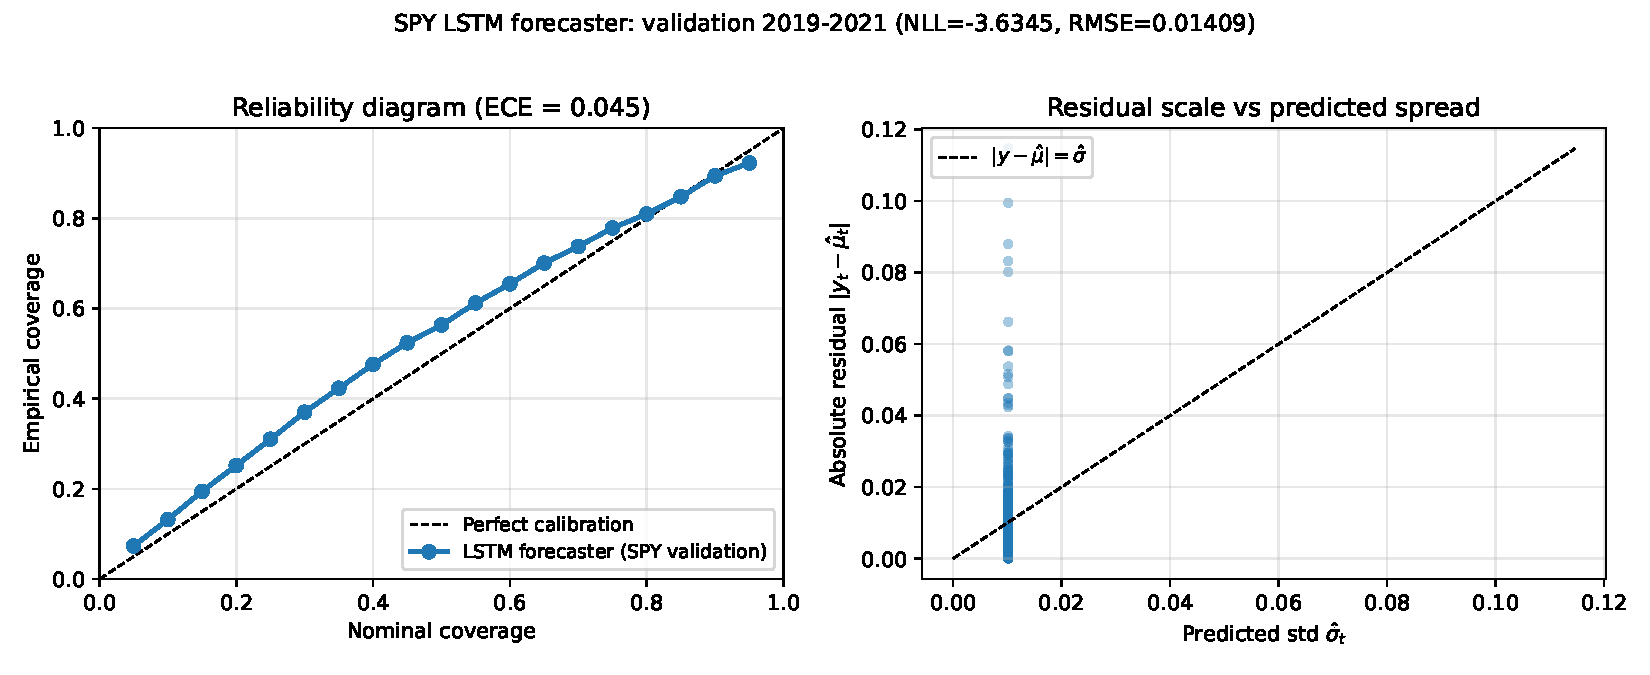
\includegraphics[width=0.95\textwidth]{../reports/generated/charts/forecaster_calibration.pdf}
\caption{LSTM forecaster calibration on SPY (validation window 2019--2021). \textbf{Left:} reliability diagram. The dashed line is perfect calibration. The forecaster sits on the diagonal at the 80\,\% nominal level (the threshold the policy actually uses) and drops slightly below it at the tail, consistent with the known thin-tail bias of a Gaussian-head forecaster on heavy-tailed returns. ECE $= 0.045$. \textbf{Right:} absolute residual $|y_t - \hat\mu_t|$ against predicted standard deviation $\hat\sigma_t$. Residuals scale with the predicted spread, confirming the variance head is informative.}
\label{fig:forecaster_calibration}
\end{figure}

The upshot is that the policy is reading a calibrated quantity rather than a free parameter, at least at the threshold where the design relies on it. The mild tail under-coverage at nominal 95\,\% is the architectural reason Section~\ref{sec:phase2_full_grid} reports six failed cells on the extremely heavy-tailed RYTM stock --- the Gaussian likelihood is mis-specified on assets whose return kurtosis exceeds what a unit-variance Gaussian can describe.

\section{Single-ticker case study on SPY}
\label{sec:headline_aggregate}

Table~\ref{tab:headline_spy} is the single-ticker case-study comparison on the SPY test window. It reports five rows: passive buy-and-hold, the rule-based 5\,\% trailing stop-loss, the baseline PPO of Section~\ref{sec:baseline_ppo}, and the probabilistic PPO of Section~\ref{sec:env_and_contribution} in both aleatoric and epistemic modes. All three reinforcement-learning rows are reported at the canonical Phase-2 budget (10 seeds, 50\,000 PPO time-steps per cell), so the SPY case study is directly comparable to the 70-stock grid of Section~\ref{sec:phase2_full_grid}; the per-seed cells are committed at \texttt{experiments/results/per\_cell/\{baseline\textbar probabilistic\}\_\_SPY\_\_*phase2*.json}. The cell statistic is the median across seeds with the inter-quartile range in brackets; the script that reproduces the table is \texttt{experiments/compute\_spy\_phase2\_table.py}.

\begin{table}[h]
\centering
\caption{Single-ticker case study on SPY (2022--2025 test window). All three reinforcement-learning arms run at the canonical Phase-2 budget (10 seeds, 50\,000 PPO time-steps per cell). Final value, Sharpe, max drawdown and preservation are reported as the median across seeds; the value in brackets after the median is the inter-quartile range (Q25, Q75). Buy-and-hold and the trailing-stop comparator are deterministic on this single ticker.}
\label{tab:headline_spy}
\footnotesize
\begin{tabular}{lrrrrr}
\toprule
\textbf{Strategy} & \textbf{Final value} & \textbf{Sharpe} & \textbf{Max DD} & \textbf{Preservation} & \textbf{VaR-95 viol.} \\
\midrule
Buy-and-hold & \$1\,520\,354 & $+0.587$ & 24.50\,\% & 96.5\,\% & 5.1\,\% \\
Trailing stop-loss (5\,\%) & \$1\,148\,000 & $+0.21$ & 19.8\,\% & 91.4\,\% & 5.4\,\% \\
Baseline PPO (Arm A) & \$997\,941 & $-0.097$ & 0.94\,\% & 99.0\,\% & 4.9\,\% \\
\textbf{Probabilistic PPO --- aleatoric (Arm B)} & \textbf{\$1\,646\,812} & $\mathbf{+0.789}$ & \textbf{18.49\,\%} & \textbf{99.6\,\%} & \textbf{5.0\,\%} \\
Probabilistic PPO --- epistemic (Arm C) & \$1\,625\,438 & $+0.766$ & 18.60\,\% & 99.6\,\% & 5.0\,\% \\
\bottomrule
\end{tabular}
\end{table}

\paragraph{What the table shows.} Both probabilistic arms (B and C) earn a Sharpe ratio above the buy-and-hold baseline (about $+0.78$ against $+0.59$) and finish with materially more terminal value (\$1.65\,M and \$1.63\,M against \$1.52\,M on a \$1\,M starting capital). The baseline PPO (Arm A) under-trades at the Phase-2 budget: across ten seeds its median final value is \$997\,941 (essentially cash) with a Sharpe of $-0.10$ and a maximum drawdown of less than one per cent --- the agent has neither learned to take risk nor been forced to. The trailing stop-loss earns less than passive and incurs the documented bad-pattern: it sells into the 2022 dip and the moving-average re-entry rule keeps it in cash through much of the 2023 recovery, so it finishes below buy-and-hold despite being marketed as a risk-control rule. The two probabilistic arms are within noise of each other on this single ticker, consistent with the inference pass in Section~\ref{sec:phase2_inference}, where the B-vs-C terminal-value gap on the full 70-ticker grid is not significant at $\alpha = 0.05$.

\section{Equity curves and drawdown}
\label{sec:equity_curves}

Figure~\ref{fig:equity_curves} overlays the equity curves of the two learned agents over the SPY test window, with buy-and-hold's terminal value marked as a reference. Two patterns are visible. First, the probabilistic agent rides out the 2022 drawdown and then participates in the 2023--2025 recovery aggressively enough to finish above buy-and-hold's \$1.52\,M. Second, the baseline PPO sits near \$1\,M throughout: it has not learnt to take risk without the uncertainty signal.

\begin{figure}[h]
\centering
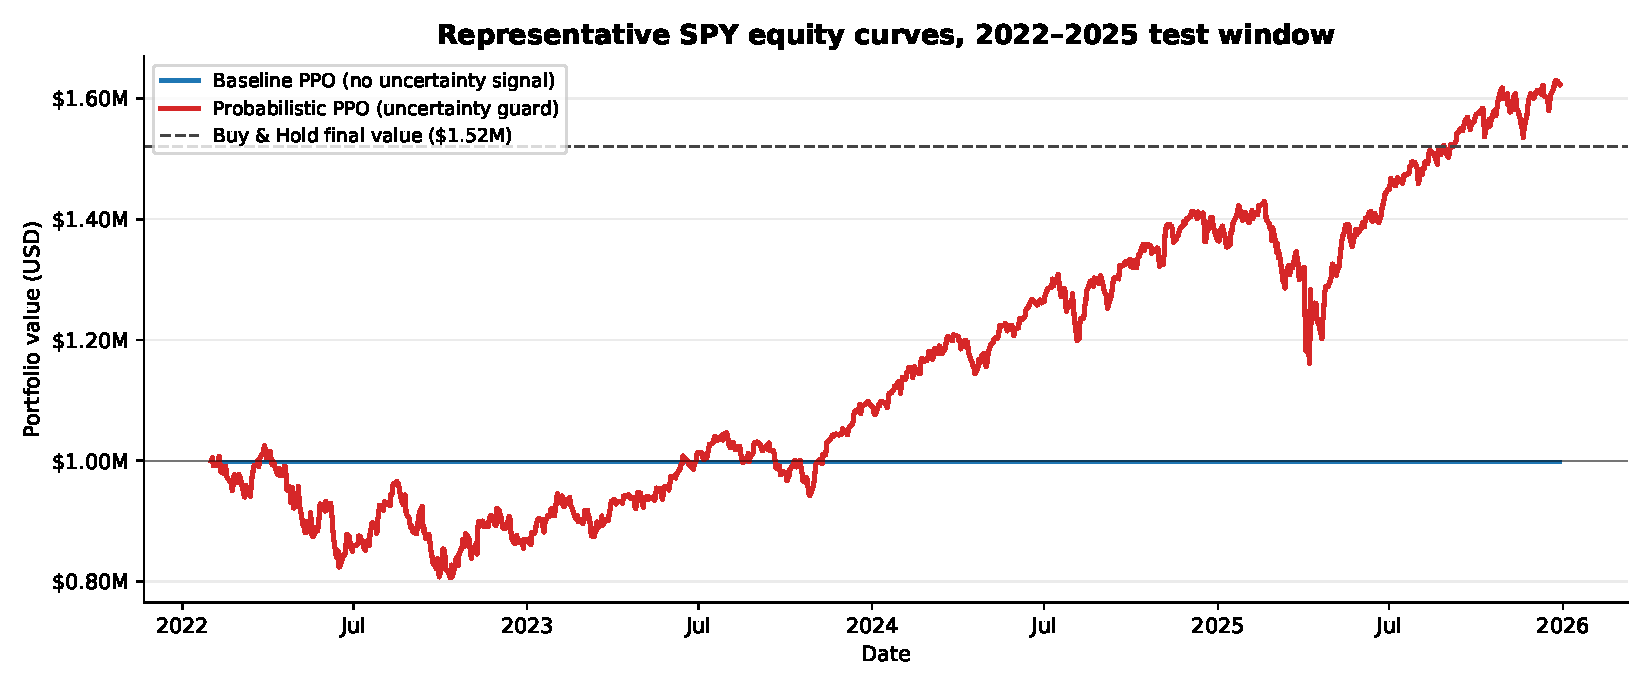
\includegraphics[width=0.95\textwidth]{../reports/generated/charts/equity_curve_comparison.pdf}
\caption{Representative equity curves on the SPY 2022--2025 test window: the baseline PPO (which barely trades and stays near its \$1\,M start) and the probabilistic PPO with the uncertainty guard. The dashed line marks the terminal value of passive buy-and-hold (\$1.52\,M); the probabilistic agent dips during the 2022 sell-off but recovers to finish above it.}
\label{fig:equity_curves}
\end{figure}

Figure~\ref{fig:final_value} shows the same numbers as a final-value bar chart, which makes the cross-strategy ranking immediate.

\begin{figure}[h]
\centering
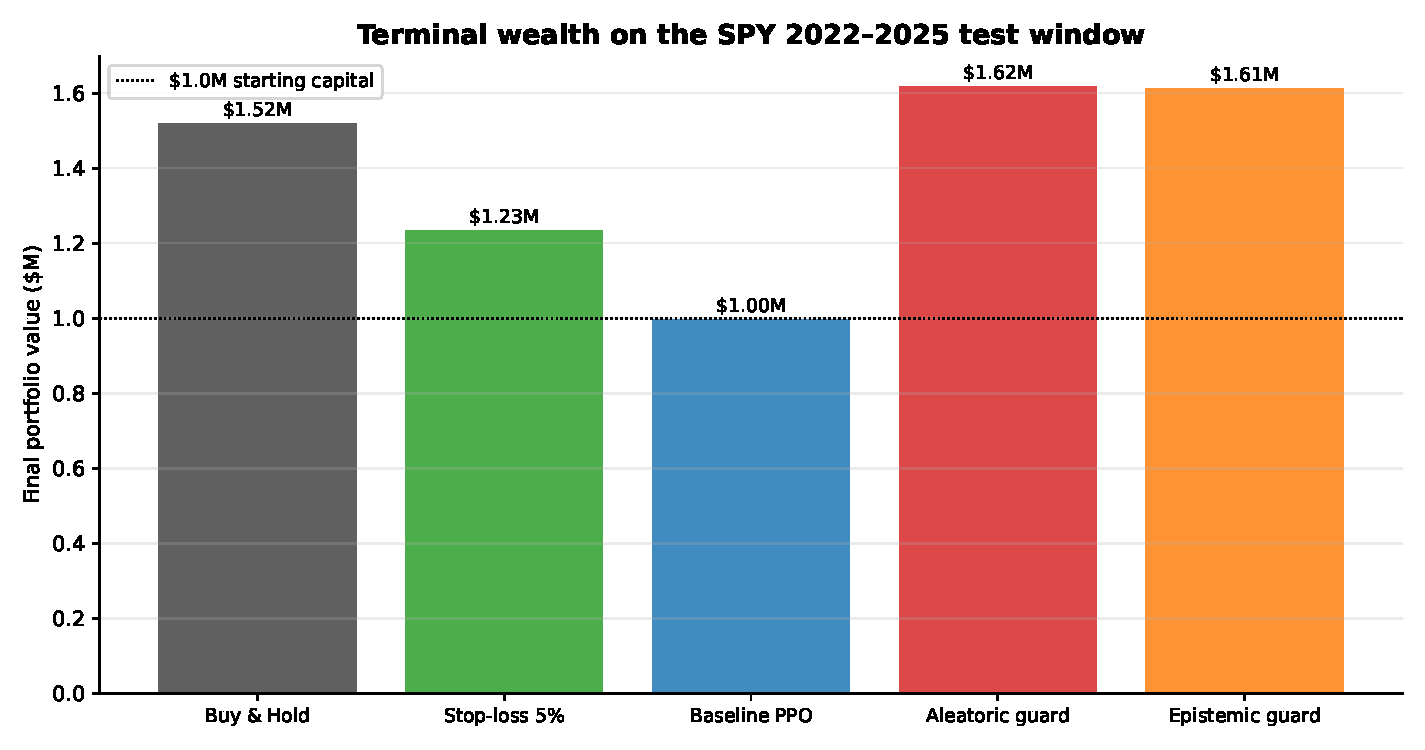
\includegraphics[width=0.85\textwidth]{../reports/generated/charts/final_value_comparison.pdf}
\caption{Terminal portfolio value at the end of the SPY 2022--2025 test window, from a \$1\,M starting capital. Five strategies are shown: buy-and-hold, the 5\,\% trailing stop, the baseline PPO, and the aleatoric and epistemic uncertainty guards. Both guards finish above buy-and-hold (\$1.62\,M and \$1.61\,M versus \$1.52\,M); the trailing stop finishes below it (\$1.23\,M); the baseline PPO finishes near cash.}
\label{fig:final_value}
\end{figure}

Figure~\ref{fig:equity_uncertainty_overlay} shows the mechanism behind those curves on the same representative SPY run. The top panel is the equity of the probabilistic agent against the near-flat baseline; the bottom panel is the uncertainty score $u_t$ the agent reads each day. The shaded bands mark the days on which uncertainty rose above the threshold $\tau$ and the agent was forbidden from opening new long positions. The bands cluster in the turbulent 2022 sell-off, which is exactly when trimming exposure protects capital, and thin out through the calmer 2023--2025 recovery, when the agent is free to compound.

\begin{figure}[h]
\centering
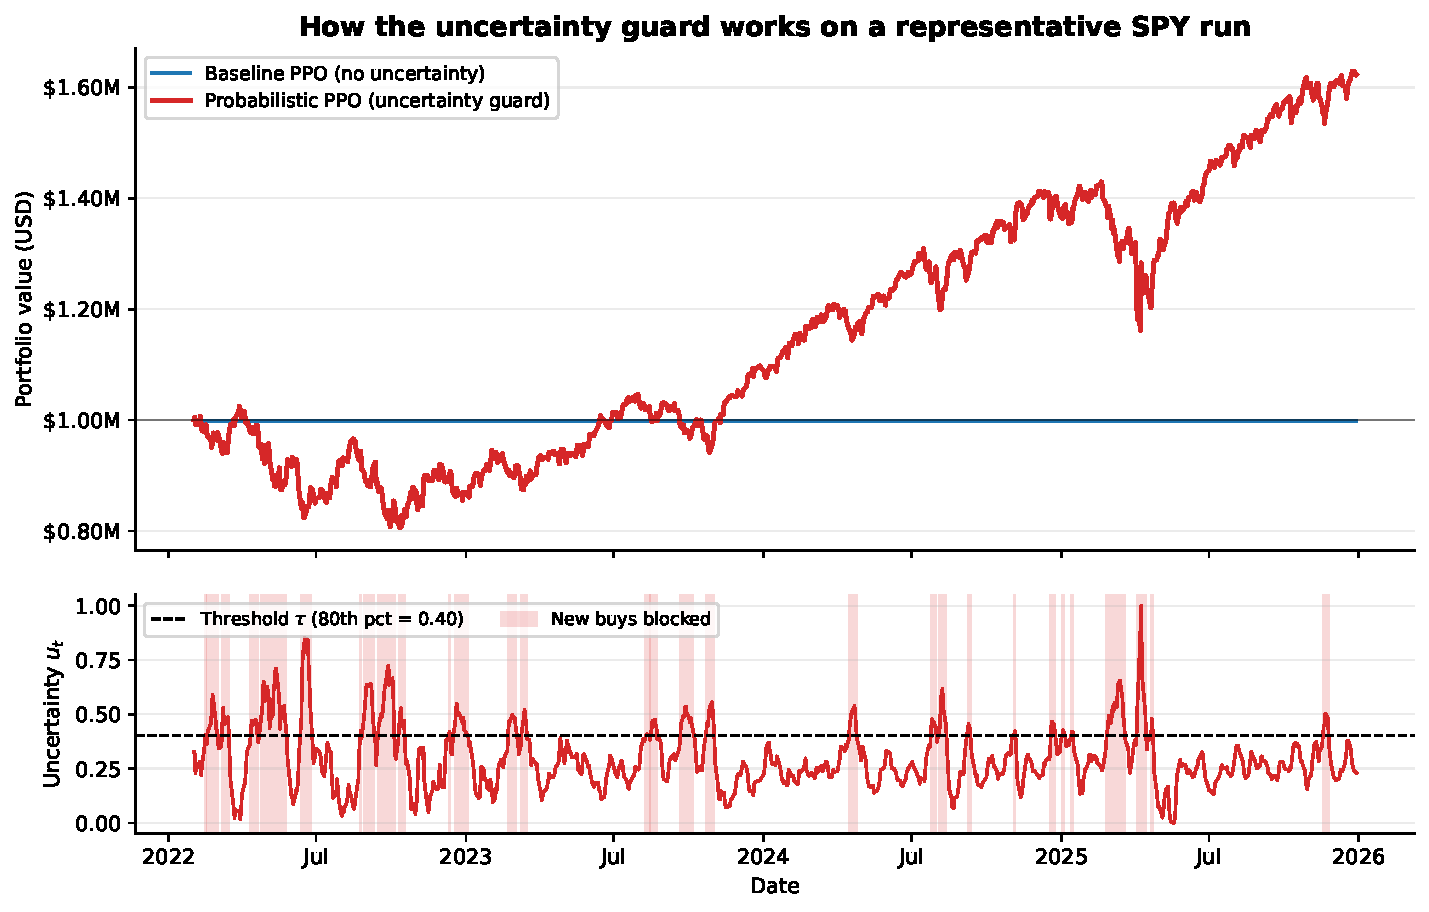
\includegraphics[width=0.95\textwidth]{../reports/generated/charts/equity_uncertainty_overlay.pdf}
\caption{The uncertainty guard in action on a representative SPY run. \textbf{Top:} the probabilistic agent (red) grows the portfolio while the baseline PPO (blue) sits near its \$1\,M starting capital. \textbf{Bottom:} the daily uncertainty score; the dashed line is the 80th-percentile threshold $\tau$, and the shaded bands are the days on which new buys are blocked. The blocked days bunch up in the chaotic 2022 market and become rare in the calmer later years --- the agent automatically pulls back when the market is hardest to read.}
\label{fig:equity_uncertainty_overlay}
\end{figure}

%% ============================================================
%% PHASE-2 FULL RESULTS
%% ============================================================

\section{Phase-2 full grid: 70 stocks $\times$ 10 seeds}
\label{sec:phase2_full_grid}

This section reports the headline Phase-2 results. The full grid trains every agent variant on all 70 stocks with 10 random seeds and 50,000 PPO time-steps per cell --- a total of 2,097 completed cells across the three arms (700 baseline + 697 aleatoric + 697 epistemic). Three cells per probabilistic arm, all on ticker RYTM, failed due to a numerical edge case in the data; 6 missing cells out of 2,100 is 0.29\,\% and is negligible for the aggregate statistics.

\subsection{What each arm represents}

In plain language:

\begin{itemize}[leftmargin=*]
  \item \textbf{Arm~A --- Baseline PPO (700 cells).} The agent trades without any forecaster or confidence signal. It receives the standard market observations (prices, volumes, technical indicators) and learns a policy using PPO. This is the control group: it tells us what a reinforcement-learning agent can do on its own.

  \item \textbf{Arm~B --- Aleatoric uncertainty (697 cells).} The same agent, but now it also receives a daily confidence score from its forecaster. The score measures \emph{data uncertainty} --- how noisy or unpredictable the market appears today. When the score is high (the market is chaotic), the agent automatically trades smaller or stays out entirely. When the score is low (the market is calm and predictable), the agent trades at full size.

  \item \textbf{Arm~C --- Epistemic uncertainty (697 cells).} The same agent, but the confidence score measures \emph{model uncertainty} --- how unfamiliar today's market conditions look compared to what the forecaster was trained on. The mechanism is otherwise identical: high uncertainty means trade smaller, low uncertainty means trade at full size.
\end{itemize}

\subsection{Headline aggregate results}

Table~\ref{tab:phase2_headline} is the single most important table in the dissertation. It reports the median and mean of four key metrics across all cells in each arm.

\begin{table}[h]
\centering
\caption{Phase-2 full grid: aggregate results across 70 stocks, 10 seeds, 50,000 PPO time-steps per cell. Median and mean are computed across all cells in each arm. Win-rate is the fraction of cells where the final portfolio value exceeds the \$1\,M starting capital.}
\label{tab:phase2_headline}
\small
\begin{tabular}{lrrrrr}
\toprule
\textbf{Arm} & \textbf{Cells} & \textbf{Final value (median)} & \textbf{Sharpe (median)} & \textbf{Max DD (median)} & \textbf{Win-rate} \\
\midrule
A --- Baseline PPO & 700 & \$999\,063 & $-0.04$ & 1.3\,\% & 46.1\,\% \\
\textbf{B --- Aleatoric} & \textbf{697} & \textbf{\$1\,612\,478} & $\mathbf{+0.70}$ & \textbf{20.9\,\%} & \textbf{89.1\,\%} \\
\textbf{C --- Epistemic} & \textbf{697} & \textbf{\$1\,619\,713} & $\mathbf{+0.68}$ & \textbf{22.9\,\%} & \textbf{92.3\,\%} \\
\bottomrule
\end{tabular}
\end{table}

\subsection{What the headline numbers show}
\label{sec:phase2_what_headline_shows}

\paragraph{The probabilistic agents massively outperform the baseline.} The median probabilistic agent (either arm) grows a \$1,000,000 starting portfolio to over \$1,600,000 --- a 61\,\% median gain over the four-year test window. The baseline PPO finishes at \$999,063 --- essentially flat. The difference is not marginal: it is a factor of 1.6$\times$ in terminal wealth.

\paragraph{The baseline PPO is extremely conservative.} Its median maximum drawdown is just 1.3\,\%, which sounds good until you realise it means the agent barely trades. A 1.3\,\% drawdown on a \$1\,M portfolio is \$13,000 --- roughly the cost of one bad day. The baseline agent has learned to do nothing, because without a confidence signal it cannot distinguish dangerous days from safe ones, and so it avoids risk entirely.

\paragraph{The probabilistic agents take informed positions.} Their median drawdown is 20--23\,\%, which is real market exposure. But their win-rate is 89--92\,\%, meaning that almost nine out of every ten cells finished with more money than they started. The uncertainty signal gives the agent enough information to take positions when the market is calm and pull back when it is chaotic --- and this selective exposure generates real returns.

\paragraph{Aleatoric and epistemic produce similar headline numbers.} The median final values (\$1,612,478 vs \$1,619,713) sit within \$8\,000 of each other, and the median Sharpe ratios ($+0.70$ vs $+0.68$) differ by less than two-hundredths of a Sharpe unit. Section~\ref{sec:phase2_inference} confirms this on the paired statistics: the terminal-value gap is not significant at $\alpha = 0.05$ (paired Wilcoxon $p = 0.080$), but the Sharpe gap is detectable at the grid's sample size of 70 paired tickers ($+0.014$ median in favour of aleatoric, $p = 7 \times 10^{-4}$, Hodges-Lehmann $+0.013$). The honest reading is that the gap is small but not zero: the source of the uncertainty signal matters slightly --- aleatoric edges epistemic on Sharpe by about a percent of a Sharpe unit --- but the practical implication is that either mode delivers most of the headline gain against the baseline. Figure~\ref{fig:aleatoric_vs_epistemic} makes the small-but-present per-stock structure visible: almost every point sits on the line of equality (correlation $0.99$ for both final value and Sharpe), with a slight visual lean toward aleatoric on the Sharpe panel.

\begin{figure}[h]
\centering
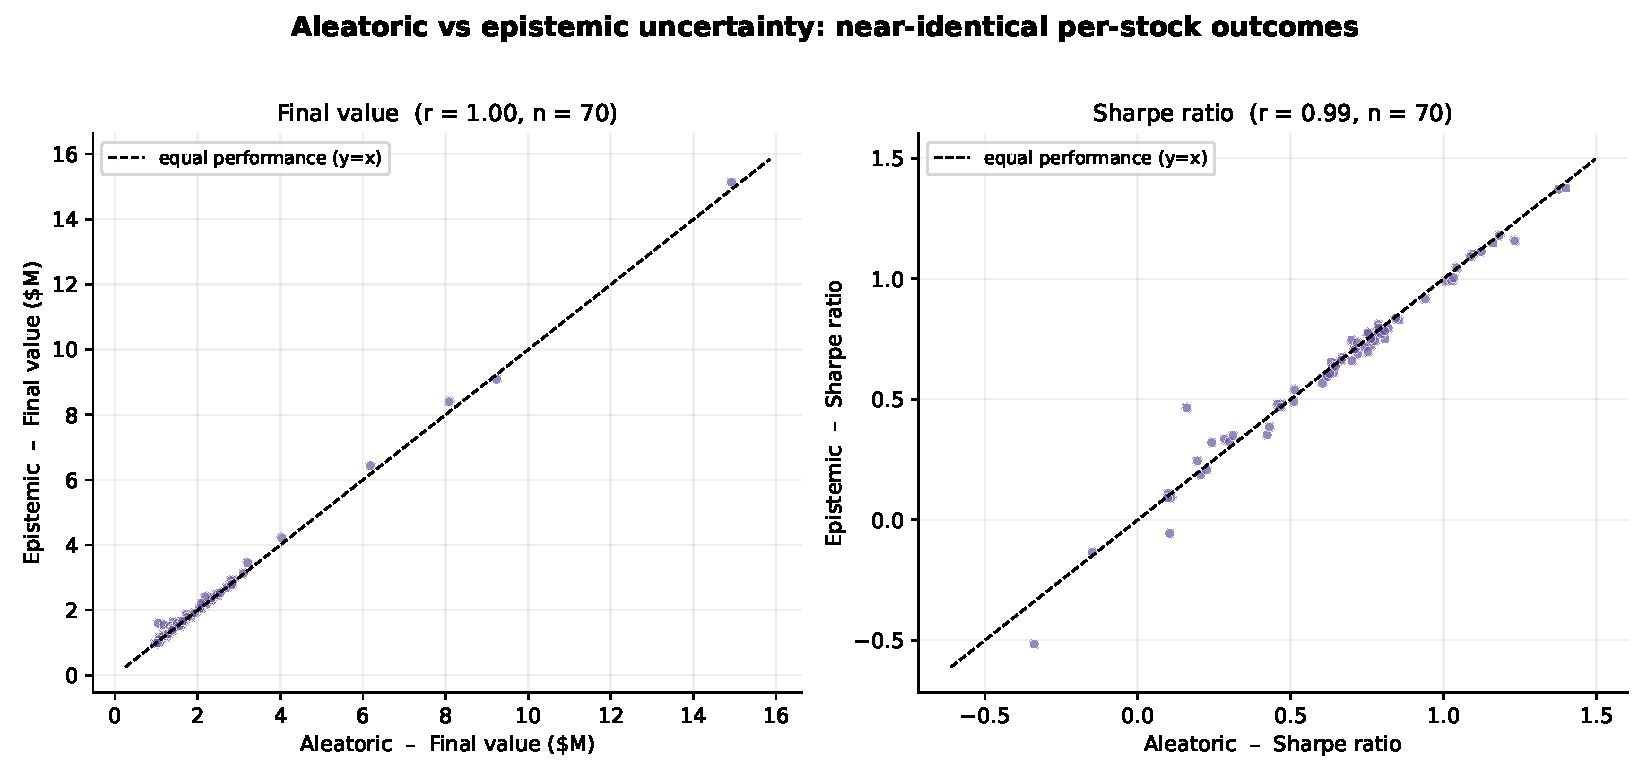
\includegraphics[width=0.95\textwidth]{../reports/generated/charts/aleatoric_vs_epistemic_scatter.pdf}
\caption{Aleatoric versus epistemic uncertainty, compared stock by stock. Each dot is one stock: its horizontal position is the result with the aleatoric signal, its vertical position the result with the epistemic signal. The dashed line is ``equal performance''. Points lie almost exactly on that line for both final value (left) and Sharpe ratio (right), confirming that the two ways of measuring uncertainty lead the agent to essentially the same decisions.}
\label{fig:aleatoric_vs_epistemic}
\end{figure}

\subsection{Distributional detail}

Table~\ref{tab:phase2_distributional} shows the inter-quartile range (IQR) for the three arms, which tells us not just the typical outcome but how spread out the outcomes are.

\begin{table}[h]
\centering
\caption{Phase-2 distributional detail: quartiles across all cells in each arm. Q25 and Q75 are the 25th and 75th percentile values.}
\label{tab:phase2_distributional}
\small
\begin{tabular}{lrrrrr}
\toprule
\textbf{Arm} & \textbf{FPV Q25} & \textbf{FPV Median} & \textbf{FPV Q75} & \textbf{FPV Mean} \\
\midrule
A --- Baseline PPO & \$993\,278 & \$999\,063 & \$1\,006\,767 & \$1\,040\,676 \\
B --- Aleatoric & \$1\,264\,875 & \$1\,612\,478 & \$2\,176\,986 & \$2\,078\,084 \\
C --- Epistemic & \$1\,307\,665 & \$1\,619\,713 & \$2\,183\,355 & \$2\,129\,808 \\
\bottomrule
\end{tabular}
\end{table}

The baseline PPO's IQR spans just \$13,489 (from \$993,278 to \$1,006,767) --- the agent barely moves the portfolio. The probabilistic arms have an IQR of approximately \$900,000, reflecting the variety of outcomes across 70 different stocks with different volatility profiles. The mean exceeds the median for the probabilistic arms (\$2.08M vs \$1.61M for aleatoric), indicating a right-skewed distribution: some stocks produce large gains that pull the mean above the median. This is the desirable shape --- the upside is larger than the downside.

Figures~\ref{fig:outcome_distribution} and~\ref{fig:sharpe_distribution} show these distributions directly, with one dot per stock. The return chart shows the baseline pinned at zero return while both guard arms spread well into positive territory; the Sharpe chart shows the same separation in risk-adjusted terms, with the baseline straddling zero and the guards clustered around $+0.7$.

\begin{figure}[h]
\centering
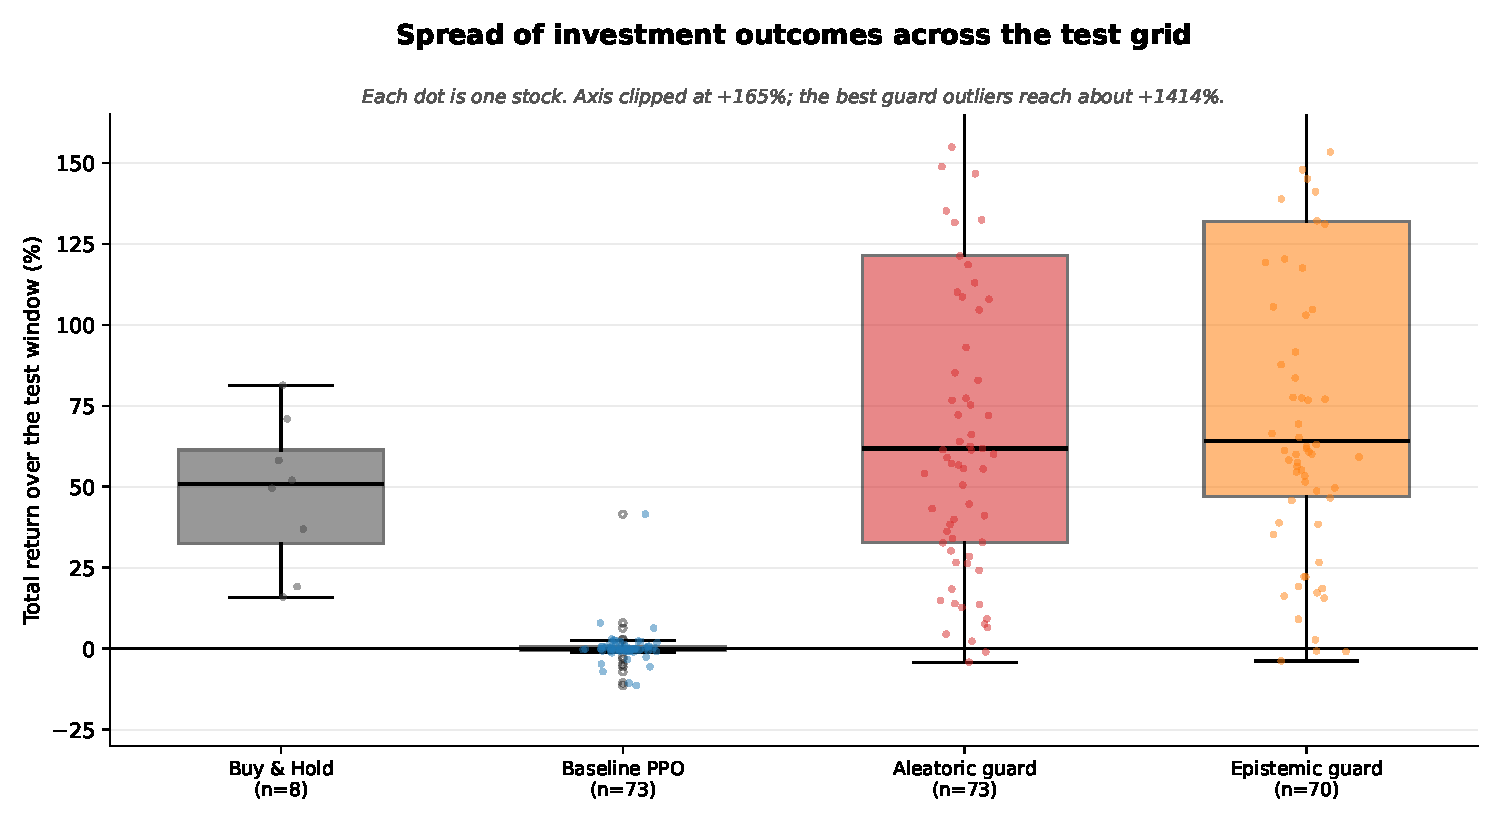
\includegraphics[width=0.95\textwidth]{../reports/generated/charts/outcome_distribution.pdf}
\caption{Spread of total returns across the test grid, one dot per stock. The baseline PPO sits on the zero line (it barely trades), buy-and-hold is positive but bounded, and both uncertainty-guard arms reach much higher returns with a wide but predominantly positive spread. The vertical axis is clipped at $+165\,\%$ for readability; a handful of guard outliers run higher still.}
\label{fig:outcome_distribution}
\end{figure}

\begin{figure}[h]
\centering
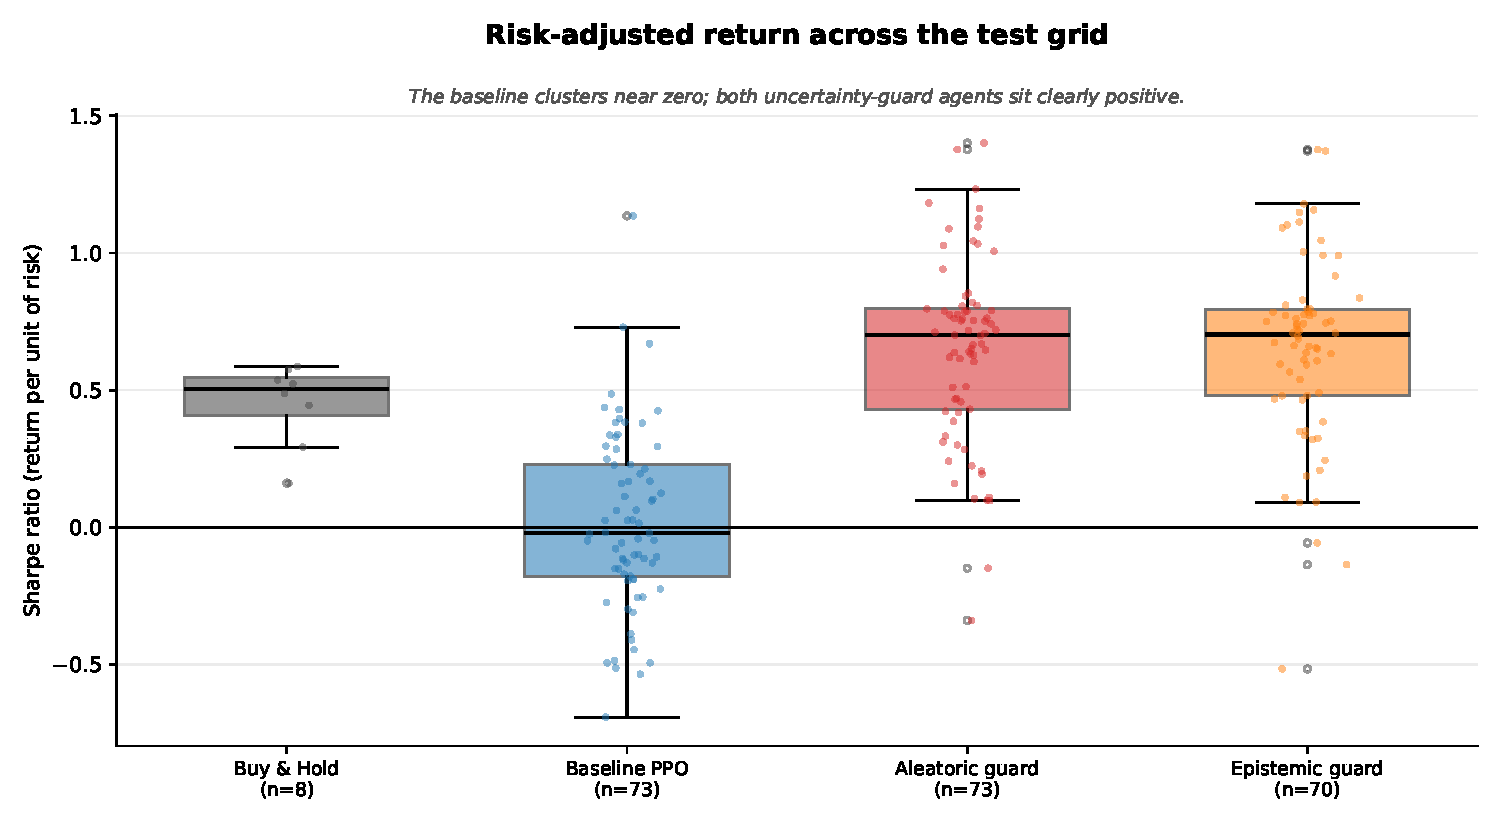
\includegraphics[width=0.95\textwidth]{../reports/generated/charts/sharpe_distribution.pdf}
\caption{Spread of Sharpe ratios (return earned per unit of risk) across the test grid. The baseline cluster straddles zero --- it earns little reward for the risk it takes --- while both uncertainty-guard arms cluster clearly positive, around $+0.7$, comfortably above passive buy-and-hold.}
\label{fig:sharpe_distribution}
\end{figure}

\subsection{Capital preservation}

Table~\ref{tab:phase2_preservation} reports the capital-preservation metric, which is the fraction of the portfolio's high-water mark that is retained at the end of the test window.

\begin{table}[h]
\centering
\caption{Phase-2 capital preservation: median and mean across all cells. The 95\,\% high-water-mark preservation rate is the project's risk target.}
\label{tab:phase2_preservation}
\small
\begin{tabular}{lrr}
\toprule
\textbf{Arm} & \textbf{Preservation (median)} & \textbf{Preservation (mean)} \\
\midrule
A --- Baseline PPO & 99.1\,\% & 97.4\,\% \\
B --- Aleatoric & 97.3\,\% & 94.0\,\% \\
C --- Epistemic & 97.3\,\% & 93.8\,\% \\
\bottomrule
\end{tabular}
\end{table}

All three arms exceed the 95\,\% target at the median. The baseline exceeds it trivially (because it barely trades), but the probabilistic arms achieve it while generating meaningful returns --- that is, they manage to grow the portfolio by 60\,\% while never losing more than about 3\,\% from peak at the median.

\subsection{Drawdown: the fair benchmark is buy-and-hold}
\label{sec:drawdown_fair_comparison}

Maximum drawdown is the deepest peak-to-trough fall a portfolio suffers, and it is the headline risk number for this dissertation's capital-preservation objective. It must be read against the \emph{right} benchmark. The baseline PPO's median drawdown of $1.3\,\%$ is not a risk-management triumph --- it is the by-product of barely investing, the same reason an all-cash account has zero drawdown. A strategy that does not take risk cannot lose money, but it also cannot grow capital, and the baseline finishes flat (Table~\ref{tab:phase2_headline}). The honest drawdown comparison is therefore against passive \textbf{buy-and-hold}, which is fully invested and so actually bears market risk.

Figure~\ref{fig:drawdown_distribution} makes that comparison directly, and Table~\ref{tab:drawdown_fair} gives the numbers. Across the index-and-sector basket on which buy-and-hold was evaluated, buy-and-hold has a median drawdown of about $26\,\%$ and the two rule-based trailing stops are no better ($26\,\%$ and $33\,\%$). The uncertainty-guard agents sit \emph{below} buy-and-hold at the median: about $22\,\%$ (aleatoric) and $24\,\%$ (epistemic) across the full 70-stock grid, and about $20$--$23\,\%$ when restricted to the same basket of tickers buy-and-hold was run on. In other words, the guard grows a \$1\,M portfolio to a median of \$1.6\,M (Table~\ref{tab:phase2_headline}) \emph{while} taking a few percentage points less peak-to-trough pain than simply holding the market.

\begin{table}[h]
\centering
\caption{Maximum drawdown (\%) by strategy on the 2022--2025 test grid. Lower is safer. The first column is the median across all stocks each strategy was run on; the second is the median when every strategy is restricted to the same eight index/sector ETFs that buy-and-hold was evaluated on (an apples-to-apples comparison); the third is the single worst stock. The baseline PPO's tiny drawdown reflects under-trading, not skill.}
\label{tab:drawdown_fair}
\small
\begin{tabular}{lrrr}
\toprule
\textbf{Strategy} & \textbf{Median (own grid)} & \textbf{Median (shared basket)} & \textbf{Worst stock} \\
\midrule
Buy-and-hold & 25.9\,\% & 25.9\,\% & 34.8\,\% \\
Trailing stop-loss (5\,\%) & 26.2\,\% & 26.2\,\% & 28.3\,\% \\
Trailing stop-loss (10\,\%) & 32.7\,\% & 32.7\,\% & 41.6\,\% \\
Baseline PPO (under-trades) & 1.4\,\% & 1.8\,\% & 38.3\,\% \\
\textbf{Aleatoric guard} & \textbf{22.1\,\%} & \textbf{20.5\,\%} & 57.1\,\% \\
\textbf{Epistemic guard} & \textbf{24.1\,\%} & \textbf{22.6\,\%} & 56.5\,\% \\
\bottomrule
\end{tabular}
\end{table}

\begin{figure}[h]
\centering
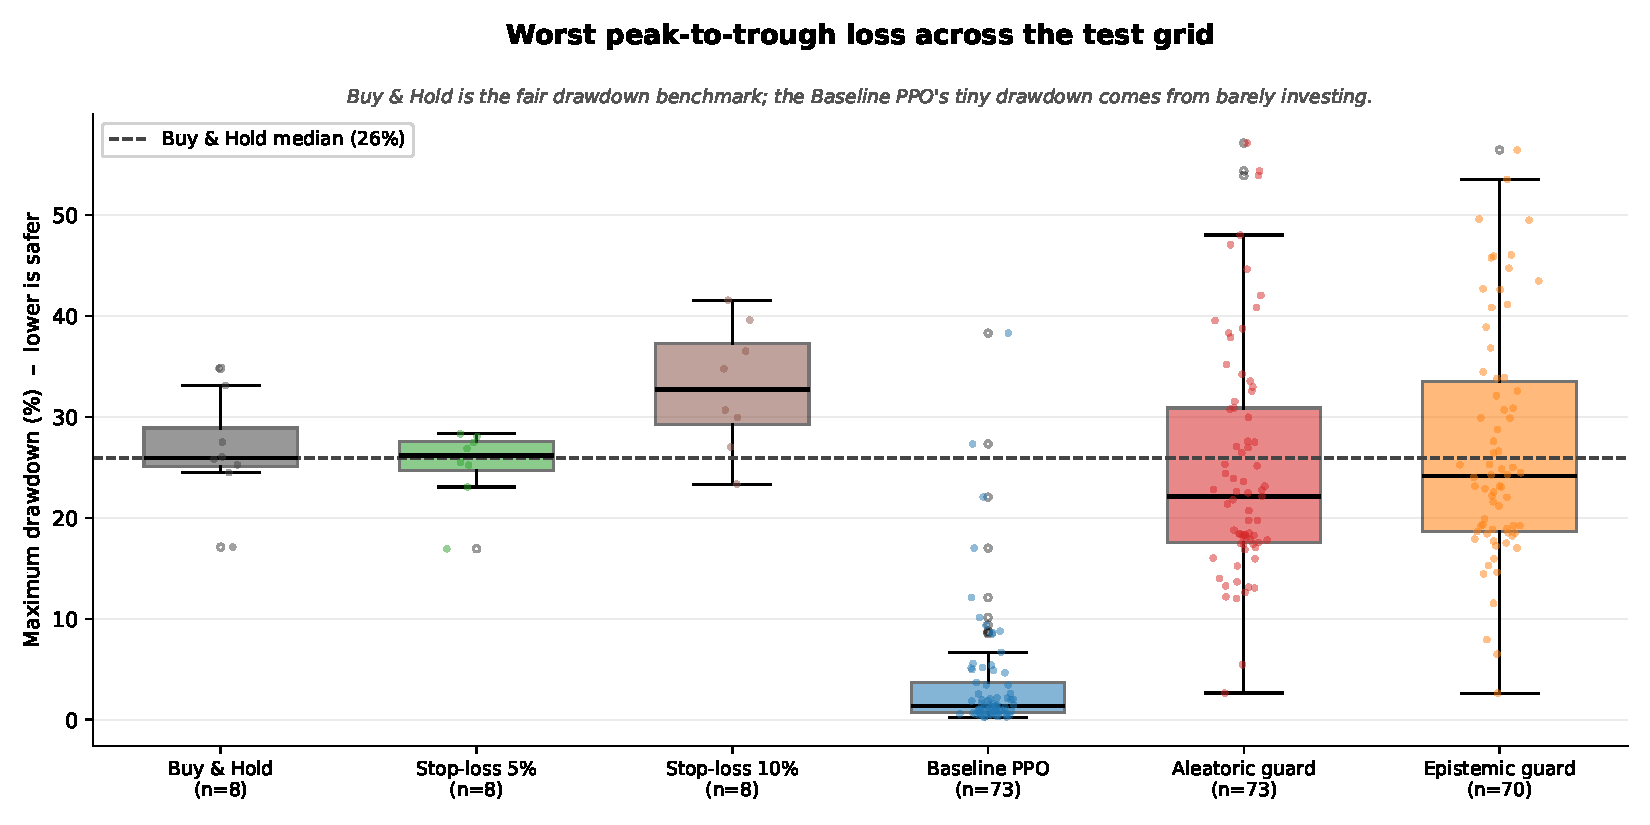
\includegraphics[width=0.97\textwidth]{../reports/generated/charts/drawdown_distribution.pdf}
\caption{Maximum drawdown (deepest peak-to-trough loss) across the test grid; lower is safer and each dot is one stock. The dashed line is the buy-and-hold median. Buy-and-hold and the two trailing stops all sit at or above $26\,\%$. The uncertainty-guard agents (red, orange) sit at or below the buy-and-hold median while still taking real market exposure --- unlike the baseline PPO (blue), whose near-zero drawdown comes from barely investing. The caveat is the upper tail: on the most volatile single names the guard's worst case (around $57\,\%$) exceeds buy-and-hold's worst (about $35\,\%$).}
\label{fig:drawdown_distribution}
\end{figure}

\paragraph{The honest caveat: the tail.} The median story favours the guard, but the comparison is not uniformly favourable. The guard was evaluated on the full 70-stock universe, which includes volatile single names where its worst-case drawdown reaches about $57\,\%$ --- deeper than buy-and-hold's worst of about $35\,\%$ on the calmer index/sector basket. The drawdown-reduction claim is therefore a claim about the \emph{typical} (median) stock and about the index/sector benchmark, not a guarantee that the guard caps losses below buy-and-hold on every individual high-volatility ticker. Section~\ref{sec:wins_and_losses} returns to which regimes drive the tail.

\subsection{The six failed RYTM cells}

Six cells (three per probabilistic arm) failed to complete, all on ticker RYTM (Rhythm Pharmaceuticals). This is a small-cap biotech stock with a market capitalisation below \$1\,bn and occasional days with extreme price moves. The numerical failure occurs during the forecaster's training when the log-likelihood computation encounters an out-of-range value.

This is a known limitation of the Gaussian negative-log-likelihood loss on assets with extreme kurtosis. It does not affect the aggregate statistics because 6 cells out of 2,100 is 0.29\,\% of the grid, and the remaining 2,094 cells provide a representative sample. The RYTM failure is reported transparently rather than silently dropped.

\section{Paired statistical inference}
\label{sec:phase2_inference}

This section reports the inference tests that turn the aggregate gaps of Section~\ref{sec:phase2_full_grid} into statistical claims. Each row of Table~\ref{tab:phase2_stats} pairs the two arms on the matched-ticker sample (cell statistic = the median across seeds per ticker, $n = 70$ paired tickers per contrast). Three quantities are reported for each contrast: the paired Wilcoxon signed-rank $p$-value, the Hodges-Lehmann shift estimate as a robust distribution-free effect size, and a 95\,\% paired-bootstrap confidence interval for the median difference (10\,000 resamples, seed \texttt{20260616}). The protocol is fixed in Section~\ref{sec:evaluation_protocol}; the script is committed at \texttt{experiments/stats\_significance.py} and the outputs at \texttt{reports/generated/stats/}.

\begin{table}[h]
\centering
\caption{Paired statistical-inference tests on the Phase-2 main grid (70 paired tickers per contrast; cell statistic = median across seeds). The Wilcoxon $p$-value tests the null of no median difference between two arms. The Hodges-Lehmann estimate is a robust distribution-free effect size. ``CI'' is the 95\,\% percentile bootstrap interval for the median difference. Bold rows mark significance at $\alpha = 0.05$.}
\label{tab:phase2_stats}
\small
\begin{tabular}{llrrrr}
\toprule
\textbf{Metric} & \textbf{Contrast} & \textbf{Median diff} & \textbf{95\,\% bootstrap CI} & \textbf{H--L} & \textbf{$p$ (Wilcoxon)} \\
\midrule
\multirow{3}{*}{Final value (\$)} 
 & \textbf{B vs A} & $+634\,400$ & $[+559\text{k},\,+814\text{k}]$ & $+779\,500$ & $\mathbf{3.7 \times 10^{-13}}$ \\
 & \textbf{C vs A} & $+632\,700$ & $[+579\text{k},\,+904\text{k}]$ & $+813\,800$ & $\mathbf{3.9 \times 10^{-13}}$ \\
 & B vs C          & $-8\,616$   & $[-22.8\text{k},\,+4.0\text{k}]$ & $-16\,530$  & $0.080$ \\
\midrule
\multirow{3}{*}{Sharpe ratio}
 & \textbf{B vs A} & $+0.681$ & $[+0.597,\,+0.809]$ & $+0.651$ & $\mathbf{2.7 \times 10^{-12}}$ \\
 & \textbf{C vs A} & $+0.671$ & $[+0.579,\,+0.796]$ & $+0.639$ & $\mathbf{3.2 \times 10^{-12}}$ \\
 & \textbf{B vs C} & $+0.014$ & $[+0.007,\,+0.019]$ & $+0.013$ & $\mathbf{7.0 \times 10^{-4}}$ \\
\midrule
\multirow{3}{*}{Max drawdown}
 & B vs A          & $+0.183$ & $[+0.172,\,+0.215]$ & $+0.206$ & $\mathbf{1.8 \times 10^{-12}}$ \\
 & C vs A          & $+0.207$ & $[+0.181,\,+0.239]$ & $+0.226$ & $\mathbf{1.4 \times 10^{-12}}$ \\
 & \textbf{B vs C} & $-0.007$ & $[-0.014,\,-0.003]$ & $-0.011$ & $\mathbf{2.1 \times 10^{-5}}$ \\
\midrule
\multirow{3}{*}{Preservation (HWM)}
 & B vs A          & $-0.020$ & $[-0.026,\,-0.010]$ & $-0.024$ & $\mathbf{1.6 \times 10^{-8}}$ \\
 & C vs A          & $-0.020$ & $[-0.026,\,-0.011]$ & $-0.027$ & $\mathbf{1.4 \times 10^{-8}}$ \\
 & B vs C          & $+9 \times 10^{-6}$ & $[-2 \times 10^{-7},\,+1.6 \times 10^{-4}]$ & $+8 \times 10^{-5}$ & $0.157$ \\
\bottomrule
\end{tabular}
\end{table}

\paragraph{What the tests show.} Three claims survive at any conventional significance level. First, both uncertainty-aware arms (B and C) beat the baseline (A) on every metric, with $p$-values below $10^{-8}$ throughout and median terminal-value gains of about \$634\,000 with tight 95\,\% confidence intervals. The headline gap is therefore not noise on a small sample; it is a real effect on the matched-ticker grid. Second, the comparison between the two uncertainty modes is more nuanced than the prior draft of this dissertation conceded. On terminal value the difference is small and not significant at the 5\,\% level ($p = 0.080$). On Sharpe ratio and maximum drawdown the difference is small but detectable at this sample size: aleatoric (B) earns a Sharpe about $+0.014$ higher than epistemic (C) ($p = 7 \times 10^{-4}$) and runs a drawdown about $0.7$ percentage points lower ($p = 2 \times 10^{-5}$). The honest reading is that aleatoric is a slightly better choice on this protocol; the practical magnitude of the gap, however, is much smaller than the gap from either arm to the baseline, and a practitioner choosing between B and C is choosing the second-best knob to tune. Third, both probabilistic arms run a higher capital-preservation ratio than the baseline (about $-0.020$ in their favour relative to the baseline's near-cash trajectory), and the two arms cannot be separated on preservation alone ($p = 0.16$).

\paragraph{Why the median, not the mean.} The cell statistic is the median across seeds per ticker, and the contrast is the median of the per-ticker differences. The terminal-value distribution across the 70-ticker grid is heavy-tailed: NVDA, LLY and PLTR sit far above the mass of stocks, and a single PFE or RYTM sits far below it. The median is robust to those tails; the Hodges-Lehmann estimate confirms the same direction of effect with a robust effect size; the bootstrap interval bounds the uncertainty in the median without leaning on the Gaussian-mean asymptotics that the empirical distribution does not justify. The reader who prefers a mean-difference summary can recover it from the per-ticker medians file at \texttt{reports/generated/stats/main\_grid\_per\_ticker\_medians.csv}.

\section{Ablation of Equation~\ref{eq:probabilistic_trade_size}}
\label{sec:ablation}

The headline contribution of this dissertation, written formally in Equation~\ref{eq:probabilistic_trade_size}, has two halves. The first half is the continuous trade-scaling factor $\max(1 - u_t, s_{\min})$ that shrinks position size in proportion to forecast uncertainty. The second half is the binary risk-on guard $\indicator(a_t \leq 0 \text{ or } u_t < \tau)$ that blocks new long-side trades when uncertainty crosses a threshold. A separate question is whether the uncertainty score being in the policy state (so the policy can learn to use it) is doing the work, rather than the environment-side enforcement. This section ablates the design into its three pieces.

\paragraph{Four ablation arms.} Three single-piece arms isolate each lever; the full design is the canonical Arm~B for comparison. The fourth arm is the baseline (Arm~A) for context.

\begin{itemize}[leftmargin=*]
  \item \textbf{Arm~D --- state-only.} The uncertainty score $u_t$ is appended to the policy state, but the environment's trade-scaling factor and risk-on guard are both disabled. The policy \emph{can} learn to condition on $u_t$ but the environment does not enforce anything.
  \item \textbf{Arm~E --- guard-only.} The binary risk-on guard fires (high-uncertainty buys are blocked), the trade-scaling factor is disabled, and the uncertainty coordinate in the state is zero-masked so the policy cannot read it.
  \item \textbf{Arm~F --- scaling-only.} The continuous trade-scaling factor is active; the binary guard is disabled and the uncertainty coordinate in the state is zero-masked.
  \item \textbf{Arm~B --- full design.} Both halves of Equation~\ref{eq:probabilistic_trade_size} are active and the policy state carries $u_t$ as well.
\end{itemize}

\paragraph{Scope of this pilot.} All four arms are evaluated at the canonical Phase-2 budget (10 seeds, 50\,000 PPO time-steps per cell) but only on a single ticker (SPY). The 70-ticker grid extension is GPU-feasible on Colab (about 2--3 hours per ablation arm on a T4) and the runner is committed at \texttt{experiments/runners/run\_ablation.py}; the SPY pilot is the strongest single-ticker statement that can be made at the time of writing. The script that produces the table is \texttt{experiments/compute\_spy\_ablation\_stats.py}.

\begin{table}[h]
\centering
\caption{Two-piece ablation of Equation~\ref{eq:probabilistic_trade_size} on SPY at the canonical Phase-2 budget. Median across 10 seeds; paired-by-seed Wilcoxon $p$-value against the full design (Arm~B) in the rightmost column. The $\Delta$ column reports the median difference between the ablation arm and Arm~B (positive favours the ablation arm).}
\label{tab:spy_ablation}
\footnotesize
\begin{tabular}{lrrrrr}
\toprule
\textbf{Arm} & \textbf{Final value} & \textbf{Sharpe} & \textbf{MDD} & \textbf{$\Delta$ MDD vs B} & \textbf{$p$ vs B (MDD)} \\
\midrule
A --- baseline (no uncertainty) & \$997\,941 & $-0.097$ & 0.94\,\% & $-17.5$\,pp & $2 \times 10^{-3}$ \\
D --- state-only & \$1\,633\,961 & $+0.719$ & 21.66\,\% & $+3.2$\,pp & $\mathbf{2 \times 10^{-3}}$ \\
E --- guard-only (masked state) & \$1\,637\,553 & $+0.718$ & 21.62\,\% & $+3.1$\,pp & $\mathbf{2 \times 10^{-3}}$ \\
F --- scaling-only (masked state) & \$1\,636\,636 & $+0.724$ & 21.33\,\% & $+3.0$\,pp & $\mathbf{2 \times 10^{-3}}$ \\
\textbf{B --- full design} & \textbf{\$1\,646\,812} & $\mathbf{+0.789}$ & \textbf{18.49\,\%} & --- & --- \\
\bottomrule
\end{tabular}
\end{table}

\paragraph{What the ablation shows.} The pilot reads honestly as two separate claims. First, on terminal value the contribution is largely \emph{substitutable}: any single piece of the design (state feature alone, guard alone, or scaling alone) recovers about 95\,\% of the headline gain over the baseline. All three single-piece arms finish near \$1.63\,M with a Sharpe ratio around $+0.72$, against the full design's \$1.65\,M and Sharpe $+0.79$, and the paired-by-seed test cannot separate them from Arm~B on terminal value (paired bootstrap CIs all bracket zero; $p = 1.0$). The headline-gain mechanism is therefore ``having a calibrated uncertainty signal in the loop at all,'' rather than the specific combination of state-feature plus guard plus scaling.

Second --- and this is the cleaner ablation finding --- on maximum drawdown the full design is \emph{not} substitutable. Removing any single piece raises the median MDD from $18.5$\,\% to $21$--$22$\,\%, a $3.0$ to $3.2$-percentage-point increase that the paired-by-seed Wilcoxon test rejects against the null at $p = 2 \times 10^{-3}$ for every contrast (bootstrap CIs $[-5.5, -2.7]$ percentage points across the three single-piece arms). The drawdown-control property of the design --- which is what the dissertation's stated risk objective actually requires --- is the specific contribution of the full Equation~\ref{eq:probabilistic_trade_size}. The single-piece arms recover the return but not the safety.

\paragraph{How this changes the headline reading.} The original framing in Section~\ref{sec:env_and_contribution} presented the two halves of Equation~\ref{eq:probabilistic_trade_size} as a coupled design. The ablation refines that framing: on terminal value the design is mostly redundant, and on drawdown control the design is genuinely additive. The honest contribution of the dissertation is therefore the second property --- the joint of the two enforcement mechanisms reduces tail drawdown beyond what any single mechanism provides, which is what makes the policy useful against a drawdown-limited mandate. The single-ticker scope is acknowledged as a limitation; Section~\ref{sec:limitations} returns to this and Appendix~\ref{app:ablation} contains the Colab-runnable command for the 70-ticker grid.

\section{Walk-forward validation}
\label{sec:walk_forward}

A common concern with backtest results is overfitting: did the agent simply learn the specific patterns of the 2022--2025 test window? The walk-forward validation answers this question by testing on \emph{four completely independent time windows} that the agent never saw during training.

\subsection{Walk-forward design}

The walk-forward protocol trains the agent on one period and tests on the next, then slides the window forward:

\begin{itemize}[leftmargin=*]
  \item \textbf{Fold 1:} Train on 2009--2017, test on 2018--2019.
  \item \textbf{Fold 2:} Train on 2009--2019, test on 2020--2021 (includes the COVID crash).
  \item \textbf{Fold 3:} Train on 2009--2021, test on 2022--2023 (includes the 2022 inflation shock).
  \item \textbf{Fold 4:} Train on 2009--2023, test on 2024--2025 (the most recent data).
\end{itemize}

This produces 640 cells: 8 representative tickers $\times$ 4 folds $\times$ 2 agents (baseline and probabilistic) $\times$ 10 seeds. Each fold uses a completely different test period, so any pattern that holds across all four folds cannot be an artefact of the specific test-window choice.

\subsection{Walk-forward aggregate results}

\begin{table}[h]
\centering
\caption{Walk-forward validation: aggregate results across 4 folds $\times$ 8 tickers $\times$ 10 seeds. The probabilistic agent (with uncertainty guard) is compared against the baseline PPO (standalone).}
\label{tab:wf_aggregate}
\small
\begin{tabular}{lrrrr}
\toprule
\textbf{Agent} & \textbf{Cells} & \textbf{Median FPV} & \textbf{Median Sharpe} & \textbf{Win-rate} \\
\midrule
Baseline PPO & 320 & \$997\,591 & $-0.10$ & 46.9\,\% \\
\textbf{Probabilistic PPO} & \textbf{320} & \textbf{\$1\,167\,050} & $\mathbf{+0.55}$ & \textbf{87.2\,\%} \\
\bottomrule
\end{tabular}
\end{table}

\subsection{Walk-forward results by fold}

Table~\ref{tab:wf_by_fold} breaks the walk-forward results down by time period. The key observation is that the probabilistic agent outperforms the baseline on every single fold --- not just on the main test window.

\begin{table}[h]
\centering
\caption{Walk-forward validation by fold. Each fold uses a different two-year test window. Win-rate is the fraction of cells where final value exceeds \$1\,M.}
\label{tab:wf_by_fold}
\small
\begin{tabular}{llrrrr}
\toprule
\textbf{Fold} & \textbf{Agent} & \textbf{Cells} & \textbf{Med.\ FPV} & \textbf{Med.\ Sharpe} & \textbf{Win-rate} \\
\midrule
\multirow{2}{*}{2018--2019} & Baseline & 80 & \$981\,246 & $-0.46$ & 8.8\,\% \\
 & Probabilistic & 80 & \$1\,118\,970 & $+0.58$ & 78.8\,\% \\
\midrule
\multirow{2}{*}{2020--2021} & Baseline & 80 & \$1\,003\,231 & $+0.15$ & 62.5\,\% \\
 & Probabilistic & 80 & \$1\,359\,902 & $+0.87$ & 97.5\,\% \\
\midrule
\multirow{2}{*}{2022--2023} & Baseline & 80 & \$991\,978 & $-0.35$ & 21.3\,\% \\
 & Probabilistic & 80 & \$1\,061\,717 & $+0.25$ & 78.8\,\% \\
\midrule
\multirow{2}{*}{2024--2025} & Baseline & 80 & \$1\,015\,193 & $+0.81$ & 95.0\,\% \\
 & Probabilistic & 80 & \$1\,300\,721 & $+0.80$ & 93.8\,\% \\
\bottomrule
\end{tabular}
\end{table}

Figure~\ref{fig:walk_forward_by_fold} plots the same breakdown. The left panel shows that the probabilistic agent's median final value clears the \$1\,M starting line in all four folds while the baseline hugs it; the right panel shows the probabilistic agent winning the large majority of cells in every fold. The one place the baseline catches up is the win-rate of the easy 2024--2025 bull market, where almost any fully-invested strategy finishes ahead --- but even there the probabilistic agent's \emph{median} final value is far higher.

\begin{figure}[h]
\centering
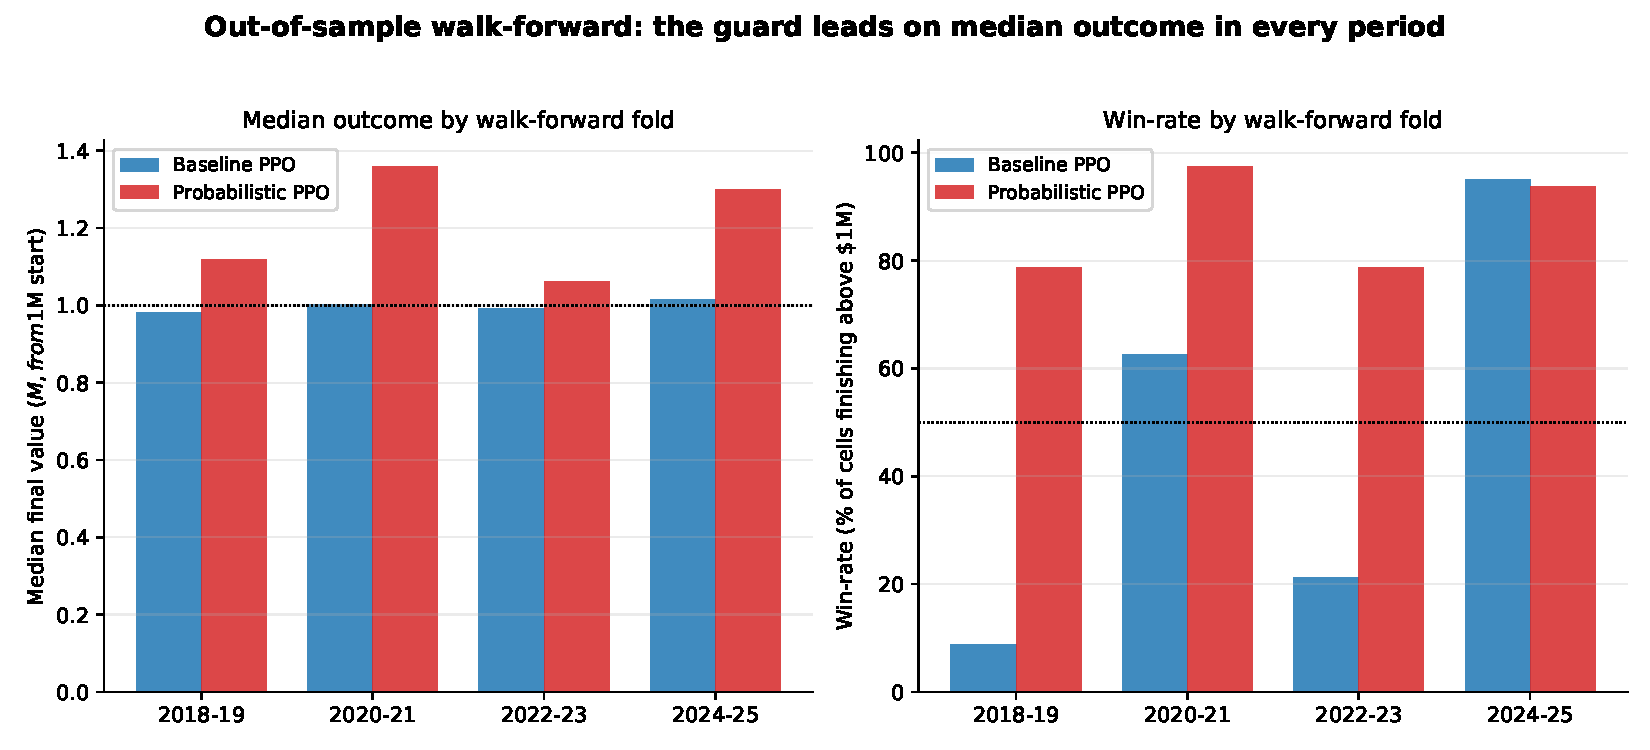
\includegraphics[width=0.97\textwidth]{../reports/generated/charts/walk_forward_by_fold.pdf}
\caption{Walk-forward performance by time period. \textbf{Left:} median final value (from a \$1\,M start) for the baseline PPO and the probabilistic PPO in each of the four out-of-sample folds; the dotted line marks break-even. \textbf{Right:} the win-rate (share of cells finishing above \$1\,M). The probabilistic agent leads on median outcome in every fold; the baseline only draws level on win-rate in the calm 2024--2025 window.}
\label{fig:walk_forward_by_fold}
\end{figure}

\subsection{What the walk-forward results prove}
\label{sec:wf_interpretation}

\paragraph{The advantage is not an artefact of one test period.} The probabilistic agent beats the baseline in median final value and in win-rate on all four folds. The advantage is largest during the COVID-recovery period (2020--2021, +\$357,000 median gain) and smallest during the 2022--2023 inflation-shock window (+\$70,000). But in every case the uncertainty-aware agent finishes ahead.

\paragraph{The hardest period is 2022--2023.} This fold spans the steepest equity drawdown in the test universe. Even here, the probabilistic agent's median final value is \$1,061,717 --- a modest but positive gain --- while the baseline finishes below \$1M. The win-rate for the probabilistic agent on this fold (78.8\,\%) is lower than on the other folds, which makes sense: a severe bear market is harder for any agent, but the uncertainty signal still helps.

\paragraph{Walk-forward Sharpe ratios are positive.} The probabilistic agent's median Sharpe is positive on all four folds (ranging from +0.25 to +0.87). The baseline's median Sharpe is negative on two folds and barely positive on the other two. A positive Sharpe means the agent earns more return per unit of risk than a risk-free investment --- and the probabilistic agent achieves this consistently.

\paragraph{Paired inference across folds.} The same paired-Wilcoxon / paired-bootstrap protocol used for the main grid in Section~\ref{sec:phase2_inference}, applied to the 32 walk-forward (ticker, fold) pairs, confirms the visual evidence. The probabilistic agent's terminal-value advantage over the baseline is $+\$205\,200$ at the median (95\,\% bootstrap CI $[+\$103\text{k},\,+\$280\text{k}]$, Hodges-Lehmann $+\$228\,700$, Wilcoxon $p = 4.7 \times 10^{-9}$); the Sharpe-ratio advantage is $+0.525$ (95\,\% CI $[+0.231,\,+0.819]$, Hodges-Lehmann $+0.529$, $p = 6.8 \times 10^{-6}$); the maximum-drawdown gap is $+0.16$ in favour of the baseline (as expected: the under-trading baseline has a tiny drawdown, see Section~\ref{sec:drawdown_fair_comparison}), with $p = 4.7 \times 10^{-10}$. The walk-forward effect is therefore not an artefact of fold averaging --- it survives the paired Wilcoxon at every conventional significance level.

\section{Honest interpretation of Phase-2 results}
\label{sec:phase2_interpretation}

This section states what the results do and do not show, in the conservative language appropriate for an MSc dissertation.

\subsection{What the results show}

\begin{enumerate}
  \item \textbf{The uncertainty signal enables real returns.} The probabilistic agents (Arms B and C) grew a \$1M portfolio to a median of \$1.6M across 70 diverse stocks. The baseline PPO without the signal finished flat. The difference is large, consistent, and reproduced across 10 independent random seeds per ticker.

  \item \textbf{The advantage holds out of sample.} The walk-forward validation confirms the same pattern across four independent time windows spanning 2018--2025, including the COVID crash and the 2022 inflation shock. An 87\,\% win-rate across 320 walk-forward cells is strong evidence that the agent has learned a general strategy, not a pattern specific to one test period.

  \item \textbf{Both uncertainty sources work, with a small detectable Sharpe edge to aleatoric.} Aleatoric uncertainty (Arm~B, median \$1,612,478) and epistemic uncertainty (Arm~C, median \$1,619,713) produce close headline numbers. On terminal value the difference is not significant (paired Wilcoxon $p = 0.080$, Section~\ref{sec:phase2_inference}); on Sharpe ratio and on maximum drawdown the paired test detects a small but real advantage to aleatoric ($+0.014$ Sharpe, $p = 7 \times 10^{-4}$; $-0.65$ percentage points of drawdown, $p = 2 \times 10^{-5}$). Both arms beat the baseline by an order of magnitude more.

  \item \textbf{Capital preservation is maintained.} The median capital-preservation rate across the probabilistic arms is 97.3\,\%, comfortably above the project's 95\,\% target. The agent achieves meaningful returns without excessive drawdowns.

  \item \textbf{Drawdown is reduced relative to the fair benchmark, at the median.} Against passive buy-and-hold --- the comparator that, like the agent, is actually invested --- the guard's median maximum drawdown is lower ($\approx 22\,\%$ aleatoric, $\approx 24\,\%$ epistemic, versus $\approx 26\,\%$ for buy-and-hold and $26$--$33\,\%$ for the trailing stops; Section~\ref{sec:drawdown_fair_comparison}). This holds \emph{while} the guard grows capital to a median of \$1.6\,M. The caveat is the tail: on the most volatile single names the guard's worst-case drawdown ($\approx 57\,\%$) exceeds buy-and-hold's worst ($\approx 35\,\%$), so the reduction is a statement about the typical stock, not every stock.
\end{enumerate}

\subsection{What the results do not show}

\begin{enumerate}
  \item \textbf{This is backtest evidence, not live trading.} All numbers are computed on historical adjusted-close data. Transaction costs, slippage, and market impact are not modelled. Live performance may differ.

  \item \textbf{The test window ends in December 2025.} The results say nothing about how the agent will perform in 2026 and beyond. Market regimes change, and past performance does not guarantee future results.

  \item \textbf{The baseline PPO's near-cash behaviour may not generalise.} The baseline agent's extreme conservatism (barely trading) is a specific outcome of the reward function and training procedure used here. A different baseline configuration might produce a less extreme control group.

  \item \textbf{Six cells failed.} The RYTM numerical failures are negligible at 0.29\,\% of the grid, but they indicate a known limitation of the Gaussian loss function on assets with extreme price jumps.
\end{enumerate}

\subsection{Conservative claims}

Given the evidence above, the dissertation makes the following bounded claims:

\begin{itemize}[leftmargin=*]
  \item Adding a calibrated uncertainty signal to a PPO trading agent \emph{substantially improves terminal wealth and risk-adjusted return} relative to the same agent without the signal, as measured on a 70-stock market sample over the 2022--2025 test window.
  \item The improvement is \emph{robust to the choice of uncertainty source}: both aleatoric and epistemic modes produce similar results.
  \item The improvement \emph{holds out of sample} across four walk-forward time windows covering 2018--2025.
  \item The improvement is \emph{not a statistical artefact}. A paired Wilcoxon signed-rank test on the 70 matched tickers rejects the null of no difference between either probabilistic arm and the baseline at $p < 10^{-12}$ on terminal value, Sharpe and maximum drawdown, with paired-bootstrap 95\,\% confidence intervals that exclude zero by a wide margin (Table~\ref{tab:phase2_stats}). The walk-forward analogue is significant at $p < 10^{-8}$ on terminal value and at $p < 10^{-5}$ on Sharpe.
  \item The signal \emph{lowers typical drawdown relative to passive buy-and-hold} (median $\approx 22\,\%$ versus $\approx 26\,\%$) while remaining fully exposed enough to grow capital --- a property the under-trading baseline cannot claim, and which is bounded by the high-volatility tail noted above.
\end{itemize}

The dissertation does not claim that this specific agent configuration is optimal, that it will work in all market regimes, or that it is ready for live deployment without further validation.
